\chapter{Исследовательская часть}

В данном разделе будут приведены примеры работы программы, и будет проведен сравнительный анализ реализованных алгоритмов по количеству потоков и по порядку графа.

\section{Технические характеристики}

Тестирование проводилось на устройстве со следующими техническими характеристиками:

\begin{itemize}
	\item операционная система: Ubuntu 20.04.1 Linux x86\_64 \cite{linux};
	\item память : 8 GiB;
	\item процессор: AMD® Ryzen™ 3 3200u @ 2.6 GHz;
	\item 4 физических ядра, 4 логических ядра \cite{amd}.
\end{itemize}

Тестирование проводилось на ноутбуке, включенном в сеть электропитания. Во время тестирования ноутбук был нагружен только встроенными приложениями окружения, а также непосредственно системой тестирования.

\clearpage

\section{Демонстрация работы программы}

На рисунке \ref{img:example} приведен пример работы программы.

\begin{figure}[H]
	\begin{center}
		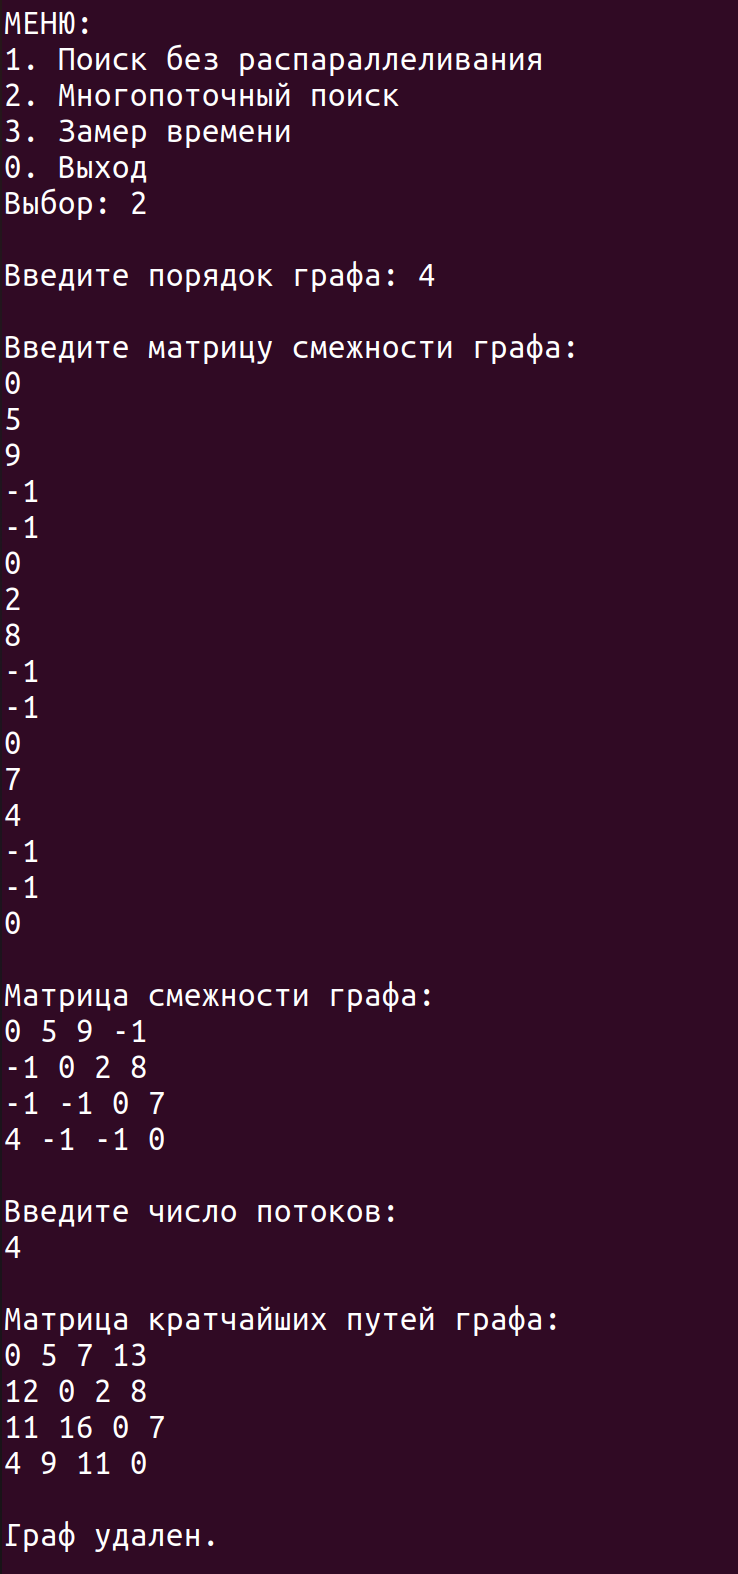
\includegraphics[scale=0.3]{img/example.png}
	\end{center}
	\captionsetup{justification=centering}
	\caption{Пример работы программы}
	\label{img:example}
\end{figure}

\section{Время выполнения алгоритмов}

Функция $std::chrono::system\_clock::now(...)$ из библиотеки $chrono$ ЯП $C++$ возвращает  процессорное время в секундах - значение типа float.

Для замера времени:
\begin{itemize}
	\item получить значение времени до начала выполнения алгоритма, затем после её окончания. Чтобы получить результат, необходимо вычесть из второго значения первое;
	\item первый шаг необходимо повторить iters раз (в программе iters равно 100), суммируя полученные значения, а затем усреднить результат.
\end{itemize}

Сравнительный анализ по времени в зависимости от количества потоков проводился для матриц смежности, заполненных случайным образом, порядком 150. Результаты измерения времени приведены в таблице \ref{tbl:time_count_threads} (в с).

\begin{table}[h]
    \begin{center}
        \begin{threeparttable}
        \captionsetup{justification=raggedright,singlelinecheck=off}
        \caption{Результаты замеров времени в зависимости от числа потоков}
        \label{tbl:time_count_threads}
        \begin{tabular}{|c|c|c|c|}
            \hline
            Кол-во потоков & С распараллеливанием  & Без распараллеливания \\
            \hline
            1 & 0.052929 & 0.055785 \\ \hline  
            2 & 0.038668 &          \\ \hline
            4 & 0.033114 &          \\ \hline
            8 & 0.037336 &          \\ \hline 
            16 & 0.035919 &          \\ \hline 
            24 & 0.037970 &          \\ \hline 
            32 & 0.036334 &          \\ \hline
		\end{tabular}
    \end{threeparttable}
\end{center}
\end{table}

На рисунке \ref{img:count_threads} приведены графические результаты сравнения временных характеристик для различного числа потоков.

\begin{figure}[H]
	\begin{center}
		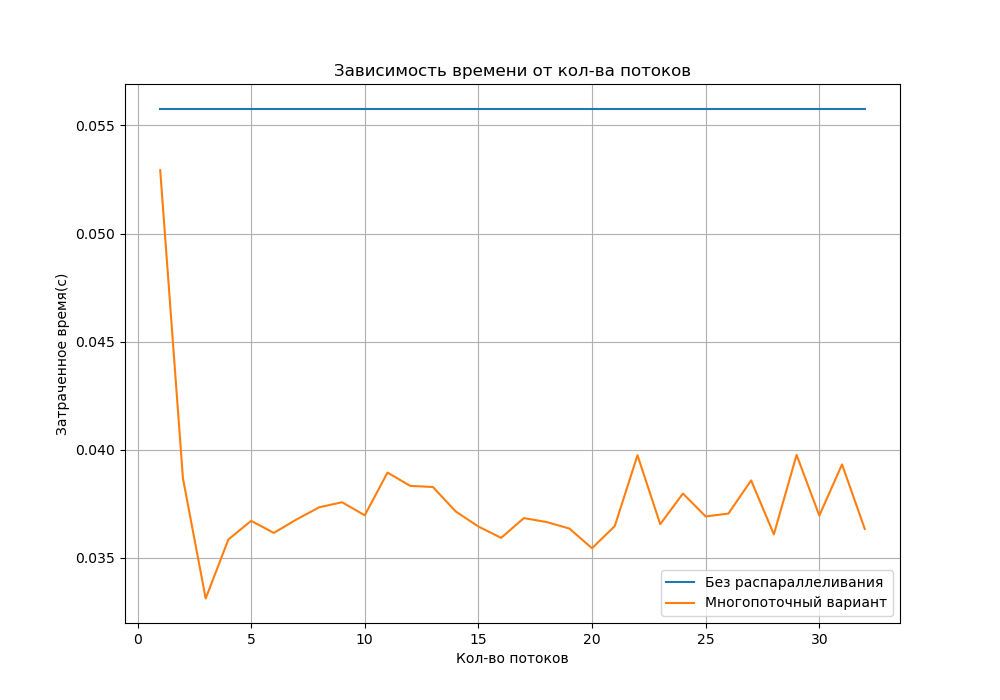
\includegraphics[scale=0.5]{img/count_threads.png}
	\end{center}
	\captionsetup{justification=centering}
	\caption{Сравнение по времени в зависимости от количества потоков}
	\label{img:count_threads}
\end{figure}

Кроме того, замеры времени проводились для матриц смежности, заполненных случайным образом, порядком от 100 до 200. Результаты измерения времени работы алгоритмов в зависимости от порядка графа приведены в таблице \ref{tbl:time_order} (в с).

\begin{table}[h]
    \begin{center}
        \begin{threeparttable}
        \captionsetup{justification=raggedright,singlelinecheck=off}
        \caption{Результаты замеров времени в зависимости от порядка графа}
        \label{tbl:time_order}
        \begin{tabular}{|c|c|c|c|}
            \hline
            Порядок & 4 потока & Без распараллеливания \\
            \hline
            100 & 0.010940 & 0.015457 \\ \hline  
            110 & 0.015257 & 0.019669 \\ \hline
            120 & 0.017407 & 0.025236 \\ \hline
            130 & 0.022600 & 0.033559 \\ \hline 
            140 & 0.026211 & 0.042147 \\ \hline 
            150 & 0.032678 & 0.058643 \\ \hline 
            160 & 0.040683 & 0.068319 \\ \hline 
            170 & 0.049890 & 0.086102 \\ \hline 
            180 & 0.060872 & 0.096152 \\ \hline
            190 & 0.070856 & 0.110270 \\ \hline 
            200 & 0.083142 & 0.130470 \\ \hline
		\end{tabular}
    \end{threeparttable}
\end{center}
\end{table}

На рисунке \ref{img:order} приведены графические результаты сравнения временных характеристик для различного порядка графа.

\begin{figure}[H]
	\begin{center}
		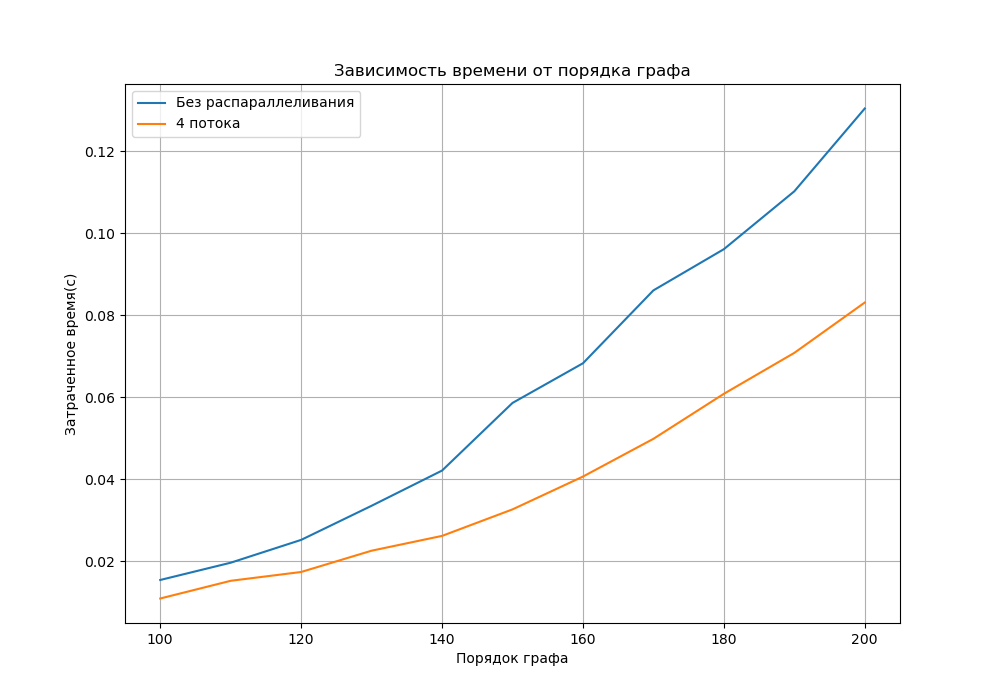
\includegraphics[scale=0.5]{img/order.png}
	\end{center}
	\captionsetup{justification=centering}
	\caption{Сравнение по времени в зависимости от порядка графа}
	\label{img:order}
\end{figure}

\section{Вывод}

В результате эксперимента было получено, что выполнение алгоритма Флойда при помощи 4 потоков быстрее его выполнения при отсутсвии многопоточности в 1.7 раза для графа порядка 150. Лучшие результаты применения многопоточности были получены при 4 потоках, так как это максимальное число потоков, допустимое на устройстве, которое было использовано для тестирования. Тогда, для указанных данных небходимо использовать параллельную реализацию алгоритма поиска кратчайших расстояний между любыми двумя вершинами.

Также в результате сравнительного анализа было установлено, что при увеличении порядка графа параллельная реализация алгоритма быстрее последовательной: при порядке, равном 120 - в 1.4 раза, при порядке, равном 200 - в 1.6 . Можно сделать вывод, что алгоритм Флойда следует параллелить при больших значениях порядка графа.